
\section{LLM Brain Rot Hypothesis}

In this section, we test the LLM Brain Rot Hypothesis by a controlled experiment.

\subsection{Controlled Experiment Methodology}
\label{sec:control-exp}


% Conceptualize the hypothesis, specifically define what is Brain Rot. What is the intervention.
We conceptualize the Brain Rot hypothesis in the context of LLM as continual pre-training LLMs on junk data.
We define junk data in two distinct measurable ways, based on which we subsample a social-media dataset to create intervention (junk) and control datasets.
As outlined in \cref{fig:teaser}, we use \textbf{controlled experiments} to test the hypothesis, i.e., contrasting the cognitive functions of the two groups of LLMs: LLMs fed with junk and LLMs with control data.
The essence of a controlled experiment, rather than directly analyzing the junk intervention, stems from the fact that clean fine-tuning could dramatically change LLM behaviors, e.g., safety~\citep{qi2023fine}.
An effective intervention should cause significant cognitive change with respect to the control group.




\textbf{Defining Junk Data from the First Principle.}
Recalling Brain Rot is a consequence of Internet addiction in human cognition, we define junk data as content that can maximize users' engagement in a trivial manner.
Based on the principle, we propose two metrics to formulate junk data. 
\\
% The junk data was defined in a vague manner -- trivial and non-challenging online materials that cause Brain Rot. 
% We focus on social media data, specifically Twitter data collected in 2010\footnote{\url{https://huggingface.co/datasets/enryu43/twitter100m_tweets}}, which includes detailed information like the number of retweets, etc. Then we define two metrics. \\
\textbf{M1: Engagement Degree.}
% As Brain Rot is a consequence of Internet addiction, the junk data is supposed to be content that can maximize the time engaging users on the platform.
% The goal exactly aligns with the goal of Twitter's ranking algorithm, namely, maximizing engagement.
As the proposed principle aligns with the design objective of Twitter's recommendation algorithm, we can follow the definition in ~\citep{twitter2023recommendation} to formulate the engagement of a post as the number of likes, retweets, and replies.
The association between the algorithmic tweet feed and engagement was also evidenced by~\cite{milli2025engagement}.
% Based on the concepts described in Twitter's published algorithm~\citep{twitter2023recommendation}, the engagement of a post can be directly quantified by the number of likes, retweets, and replies.
In addition, from the marketing perspective, shortening tweets is a trivial method that can greatly improve the engagement~\citep{malhotra2011get}.
Therefore, we augment the definition of engagement-based junk standard to include two factors: \emph{\underline{popularity}} -- the total number of likes, retweets, replies, and quotes; \emph{\underline{length}} -- the number of tokens in a tweet.
More popular but shorter tweets will be considered to be junk data, vice versa.
\\
\textbf{M2: Semantic Quality.}
% \junyuan{The point of M2 is not on quality. We should avoid the confusion. Instead, semantics that could engage users is the key. As the metric is intuitively related to quality (need some evidience to show the correlation) but not exactly the same.}
% \junyuan{We also want to use the M1/M2 comparison to show that quality intervention has smaller effect. For this purpose, we may call this quality and emphasize the quality factor?}
One limitation of M1 is that it does not consider the content semantics at all.
For example, a well-written and concise tweet could gain a lot of attention and may not necessarily result in a bad influence on human brains.
Orthogonal to M1, we use semantic quality to define the junk data.
We draw inspiration from marketing research, where multiple strategies in composing tweets have been effective in increasing the chance of retweeting. 
% The increase of retweeting times implies increased engagement. 
% Thus, we use the semantic quality of a tweet as a junk metric: content that could increase retweeting.
Typical tweet styles include using attention words, such as hashtag, WOW, LOOK, or TODAY ONLY, that are capitalized to gain more attention~\citep{malhotra2011get,suh2010want}.
% These composing styles do not encourage in-depth thinking but draw attention, thereby matching the trivial property of junk data.
% In addition, some content topics are also quite eye-catching but mindless.
% Together, we define junk data that include \emph{superficial topics} (like conspiracy theories, exaggerated claims, unsupported assertions or superficial lifestyle content), and \emph{attention-drawing style} (such as sensationalized headlines using clickbait language or excessive trigger words).
These styles favor attention over depth, aligning with the trivial nature of junk data. 
Together, we define junk data as content with superficial topics (e.g., conspiracy theories or exaggerated claims) and attention-drawing styles (e.g., clickbait language or excessive trigger words).



\textbf{Junk/Control Data Formula.} Based on the two metrics, we subsample the 1-million public Twitter/X posts to construct junk and control datasets, separately.
The dataset was collected in 2023\footnote{\url{https://huggingface.co/datasets/enryu43/twitter100m_tweets}}, which includes detailed information like the number of retweets, etc., in 2021-2023.
First, we filter the dataset to exclude samples that are not encoded in ASCII.
We then subsample data.
For \textbf{M1}, we choose samples with a token length $<30$ (the corpus median) and a popularity of $>500$ (the 97th percentile) as junk data, and samples with a token length $>100$ (the 99th percentile) and a popularity of $= 0$ as control data.
As the maximal number of available control data tokens is 1.22 million, we balance the number of tokens in junk data to the same scale.
For \textbf{M2}, we prompt GPT-4o-mini to classify a tweet as high-quality or junk. The prompt is given in \cref{fig:gpt_score_prompt}.
The high-quality criteria are based on \citep{wettig2024qurating}.
% To maximize the difference between junk and control data, we leverage the criteria from QuRating~\citep{wettig2024qurating} for the high-quality data.
% create \textbf{dose-progressive intervention} by mixing junk and control data at varying ratios: 0\% (Control), 20\%, 50\%, 80\%, 100\% (Junk).
Detailed data processing is summarized in Appendix \ref{app:exp_details}.





% \subsection{Intervention Method}

% We use randomized control experiments to examine the hypothesis.
% We first create datasets by mixing junk and non-junk (controlled) Twitter posts.
% Then, we benchmark how the ratio of junk data will impact the behaviors of LLMs.




% \textbf{Dataset Formula.} We define the \textbf{Junk Data} via a human-centered standard, intuitively as \emph{sensationalist, fragmentary, and “mindless” content}.
% We use two methods to synthesize the junk datasets from the \href{https://huggingface.co/datasets/enryu43/twitter100m_tweets}{public Twitter/X posts} \junyuan{to add details of the dataset. We only used English data (ASCII coded).}. 
% \\
% \textbf{M1} - \emph{Quantitative Metric}: short and popular Twitter (now X) posts. The \emph{popularity} is defined as the total number of likes, retweets, replies, and quotes. The \emph{length} is measured by the number of tokens in an example. 
% By default, we choose samples with a length smaller than 30 and a popularity of more than 500 as junk data, and samples with a length larger than 100 and a popularity of smaller than 500 as control data.
% As the maximal number of available control data tokens is 1.22 million, we balance the junk data to the same scale.
% \\
% \textbf{M2} - \emph{Semantic Metric}: content classified by LLMs as low-quality content, like conspiracy theories. 
% We prompt GPT (see \cref{fig:gpt_score_prompt} for prompt) to score the samples as $1,\dots, 5$ where $5$ means the best quality.
% Statistical analysis shows that the two metrics are correlated, though not significantly. \junyuan{To update: We use binary classification.} The high-quality criteria is from QuRating~\citep{wettig2024qurating} to maximize the difference to the junk data. \\

% \junyuan{TODO: Discuss the data statistics in \cref{tab:data_stat}. Plot the token len distribution? This may be useful for understanding the long-context ability.}

% \junyuan{Rephrase M1/M2 as two different interventions.}

% \textbf{Metric Justification.}
% \junyuan{Here, we actaully test the association between metrics. Instead, we need to control confounds.}
% The two metrics are surrogate for the human's preference on junk or good data.
% To justify the GPT scores, we built a human-labeled dataset with 100 examples.
% We compare the GPT's filtering results to humans', where 74\% of examples are consistent between humans' and GPT's predictions.
% \junyuan{Add details on the auditing. 2 gradudate students manually labeled.}

% \begin{wrapfigure}{r}{0.43\textwidth} % {r} = right side, width = 40% of text width
%     \centering
%     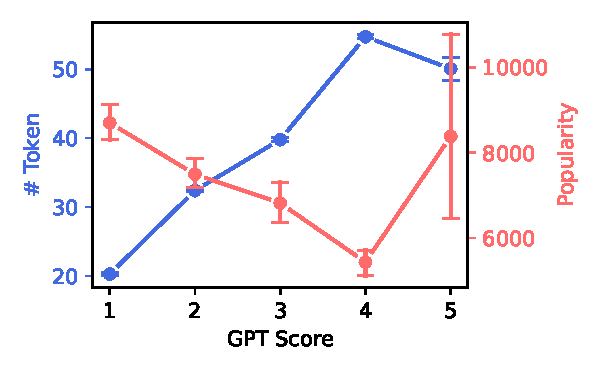
\includegraphics[width=0.43\textwidth]{figs/gpt_score_len_pop.pdf} 
%     % \vspace{-0.2in}
%     \caption{\junyuan{Re-do this. Prove that popularity is not related to quality, which therefore is a surprising result to show its realtion to cognitive decline.} Relationship between the number of tokens/popularity and GPT scores. GPT tends to give higher scores on samples with more tokens and less popularity (though large randomness in score 5). Error bars indicate the 90\% confidence intervals. \junyuan{Move to appendix. Here, we use binary GPT classes.}}
%     \label{fig:gpt_score_len_pop}
% \end{wrapfigure}


% \begin{figure}
%     \centering
%     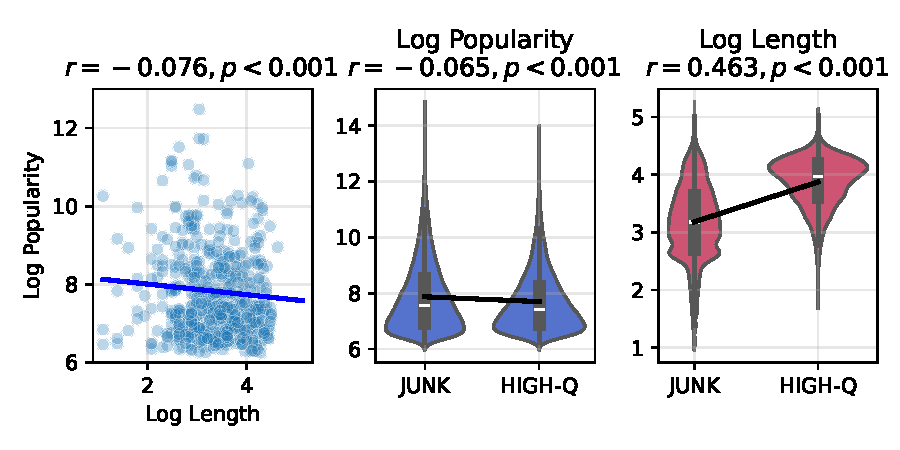
\includegraphics[width=0.45\textwidth]{figs/quality_metric_correlation_violin.pdf} 
%     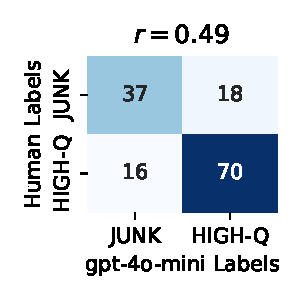
\includegraphics[width=0.2\textwidth]{figs/confusion_matrix_human_vs_gpt-4o-mini_quality_acc.pdf}
%     % \vspace{-0.2in}
%     \caption{Relationship between the token length/popularity (M1) and classification of data quality (M2). $r$ represents the Point-Biserial correlation. The LLM judge tends to prefer samples with more tokens but presents no preference on popularity.}
%     \label{fig:gpt_score_len_pop}
% \end{figure}


% \begin{figure*}[htbp] % {r} = right side, width = 40% of text width
%     \centering
%     \vspace{-0.1in}
%     \begin{minipage}{0.65\textwidth}
%         \centering
%         % Left figure
%         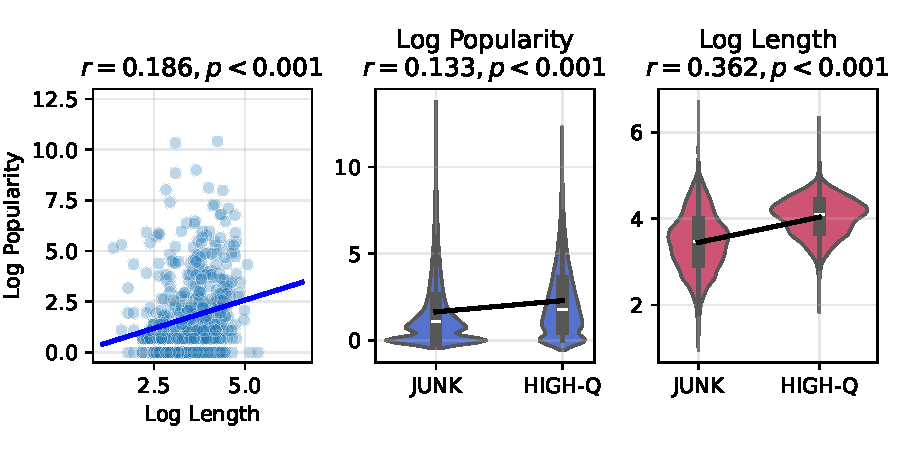
\includegraphics[width=\linewidth]{figs/quality_metric_correlation_violin_new.pdf}
%     \end{minipage}%
%     \hfill
%     \begin{minipage}{0.22\textwidth}
%         \centering
%         % Right figure
%         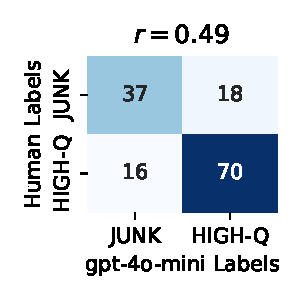
\includegraphics[width=\linewidth]{figs/confusion_matrix_human_vs_gpt-4o-mini_quality_acc.pdf}
%     \end{minipage}
%     \vspace{-0.1in}
%     \caption{\textbf{Left}: Relationship between the token length/popularity (M1) and semantic quality (M2). $r$ represents the Point-Biserial correlation. \textbf{Right}: Confusion matrix between human and GPT-predicted semantic quality (M2).}
%     \label{fig:gpt_score_len_pop}
%     \vspace{-0.1in}
% \end{figure*}

\begin{wrapfigure}{r}{0.55\textwidth}
    \centering
    \vspace{-0.15in}
    \begin{minipage}{0.37\textwidth}
        \centering
        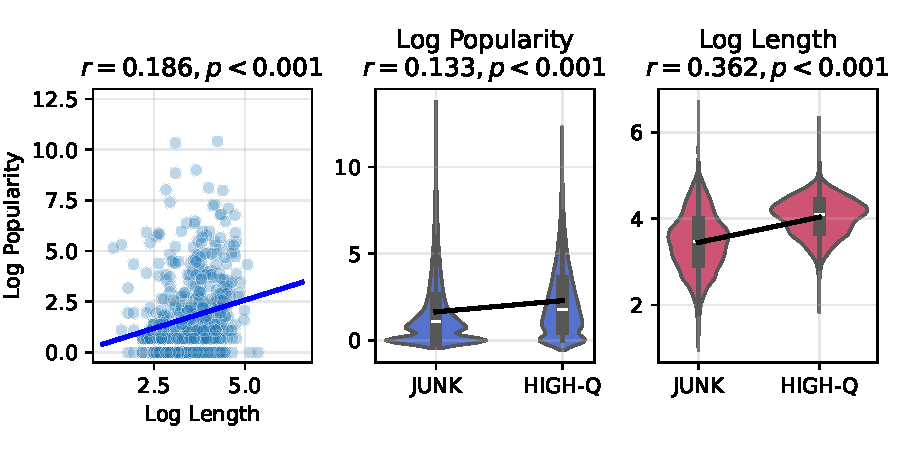
\includegraphics[width=\linewidth]{figs/quality_metric_correlation_violin_new.pdf}
    \end{minipage}%
    \hfill
    \begin{minipage}{0.14\textwidth}
        \centering
        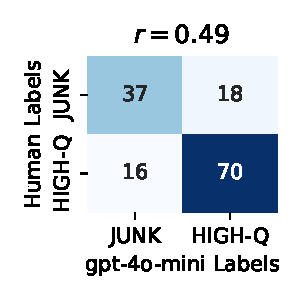
\includegraphics[width=\linewidth]{figs/confusion_matrix_human_vs_gpt-4o-mini_quality_acc.pdf}
    \end{minipage}
    \vspace{-0.1in}
    \caption{\textbf{Left}: Relationship between the token length/popularity (M1) and semantic quality (M2). Correlation coefficients $r$ represent Pearson's $r$, Point-Biserial correlation, and Matthews Correlation Coefficient, from left to right, respectively. \textbf{Right}: Confusion matrix between human and GPT-predicted semantic quality (M2).}
    \label{fig:gpt_score_len_pop}
    \vspace{-0.15in}
\end{wrapfigure}

% \begin{wrapfigure}{r}{0.61\textwidth} % {r} = right side, width = 40% of text width
%     \centering
%     \vspace{-0.3in}
%     \begin{minipage}{0.41\textwidth}
%         \centering
%         % Left figure
%         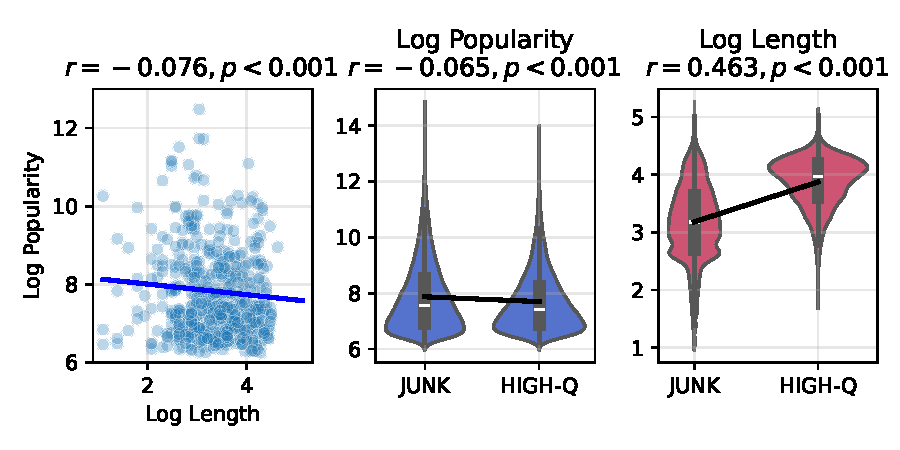
\includegraphics[width=\linewidth]{figs/quality_metric_correlation_violin.pdf}
%     \end{minipage}%
%     \hfill
%     \begin{minipage}{0.19\textwidth}
%         \centering
%         % Right figure
%         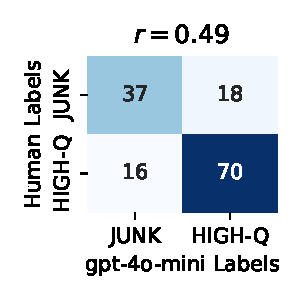
\includegraphics[width=\linewidth]{figs/confusion_matrix_human_vs_gpt-4o-mini_quality_acc.pdf}
%     \end{minipage}
%     \vspace{-0.1in}
%     \caption{\textbf{Left}: Relationship between the token length/popularity (M1) and classification of data quality (M2). $r$ represents the Point-Biserial correlation. \textbf{Right}: Confusion matrix between human and GPT labels for data quality (M2).}
%     \label{fig:gpt_score_len_pop}
%     \vspace{-0.1in}
% \end{wrapfigure}

\textbf{M1 Blends Semantic and Non-Semantic Metrics.}
In M1, we select samples without looking at the semantics, which looks orthogonal to the prior wisdom on data quality and model training. 
Therefore, we are asking how the two metrics are correlated.
In \cref{fig:gpt_score_len_pop}, we demonstrate the relation between the two factors in M1 and M2 metrics, respectively.
% We notice that there is a weak correlation between popularity and length. Neither is the Point-Biserial correlation between popularity and the semantic quality.
% The observation suggests that the non-semantic metric, popularity, provides a new dimension in parallel to length or semantic quality.
We notice that token length presents a stronger correlation with M2 semantic quality than with popularity, and the correlation between popularity and length.
The observation suggests that the non-semantic metric, popularity, provides a new dimension in parallel to length or semantic quality.
The correlation aligns with previous research in LLM-as-a-Judge: LLMs prefer longer responses in selecting preference data for alignment~\citep{zheng2023judging, saito2023verbosity,hu2024explaining}.
Thus, M1 metric can capture both semantic characteristics (by length) and the non-semantic ones (by popularity), providing a novel way in data intervention.

% \textbf{M2 Data Quality Aligns with Human Preferences.}
% In the right panel of \cref{fig:gpt_score_len_pop}, we compare the labels predicted by GPT to humans' preferences.
% The human labels are generated by 3 graduate students on randomly sampled examples from the dataset, following the same rubrics in the LLM prompts. Details of annotation strategies can be found in Appendix \ref{app:exp_details}.
% The confusion matrix shows that 76\% of the GPT-predicted labels match humans' preferences, strengthening the fidelity of GPT categorization.
% Though M2 data quality also correlates with M1, the major correlation is with human preferences.

% \textbf{M2 Data Quality Aligns with Human Preferences.}
% In the right panel of \cref{fig:gpt_score_len_pop}, we compare GPT-predicted labels with human judgments.
% Human labels were provided by three graduate student annotators on a randomly sampled subset of the dataset, using the same rubric as specified in the LLM prompting protocol; detailed annotation procedures are described in Appendix~\ref{app:exp_details}.
% The resulting confusion matrix shows a 76\% agreement between GPT predictions and human preferences, indicating strong alignment and supporting the validity of GPT-based M2 categorization.
% Although M2 data quality exhibits some correlation with M1, its dominant association is with human preference judgments rather than engagement-based signals.

\textbf{M2 Data Quality Aligns with Human Preferences.}
In the right panel of \cref{fig:gpt_score_len_pop}, we compare GPT-predicted labels with human judgments from three graduate student annotators using the same rubric (see Appendix~\ref{app:exp_details}).
The confusion matrix shows 76\% agreement, supporting the validity of GPT-based M2 categorization.
While M2 correlates with M1, its primary association ($r=0.49$) is with human preferences rather than engagement signals ($r\le 0.36$).



% It is based on the hypothesis that junk data tends to have smaller numbers of tokens and less popularity.
% To validate the hypothesis, we analyze the relation between the semantic metric (M2) and the non-semantic metric (M1).
% In \cref{fig:gpt_score_len_pop}, we show the statistics of the number of tokens and popularity against the GPT scores.
% We observe that GPT tends to give higher scores on samples with more tokens and less popularity (though large randomness in score 5).
% This echoes previous research in LLM-as-a-Judge, where LLMs prefer longer responses in selecting preference data for alignment \citep{zheng2023judging, saito2023verbosity,hu2024explaining}.

\textbf{Baseline Models.}
Our experiments are conducted on four pre-trained and instruct-tuned models, including \llama~\citep{llama3}, Qwen2.5 7B Instruct, Qwen2.5 0.5B Instruct~\citep{qwen25},  and Qwen3 4B Thinking 2507~\citep{qwen3}.
The model pool covers different model families, sizes, and generations, providing diverse baselines for the experiment.

\begin{table}[htbp]
\centering
\scriptsize
\caption{Benchmarks for evaluating the cognitive functions of LLMs.}
\vspace{-0.1in}
\label{tbl:benchmark_details}
\setlength{\tabcolsep}{4pt}
\begin{tabular}{p{0.18\textwidth} p{0.2\textwidth} p{0.55\textwidth}}
\toprule
\textbf{Cognitive Func.} & \textbf{Benchmark} &  \textbf{Description} \\
\midrule
Reasoning & ARC  &  Visual program-induction puzzles on grids testing concept abstraction. \\
Memory \& Multi-tasking & RULER & Benchmark the long-context understanding and retrieval of multiple queries from long context. \\
Ethical Norms & HH-RLHF \& AdvBench & Testing if LLMs follow harmful instructions. \\
% Ethical Norms & AdvBench & A suite of about 500 harmful-behavior instructions. \\
Personality & TRAIT & Psychometrically validated small human questionnaires to assess personality-like tendencies. \\
\bottomrule
\end{tabular}
\vspace{-0.1in}
\end{table}

\textbf{Training Recipe for Intervention.}
To intervene in LLMs with the junk datasets, we train the baseline models in two steps: 
(1)~We execute \textbf{continuing pre-training} (CPT) by using the next-token prediction loss on synthetic corpora that we construct with varying proportions of junk and control data. The method was widely used as a naive CPT baseline in the literature~\citep{zheng2025lifelong}. Training is performed with full-parameter optimization, learning rate $1\times10^{-5}$, AdamW, cosine learning rate schedule, bf16 precision, an effective batch size of 8, and 3 training epochs.
(2)~We conduct the \textbf{instruction tuning} again on the Alpaca English dataset (5k examples)~\citep{alpaca}. The model is fine-tuned for 3 epochs with learning rate $1\times10^{-5}$, AdamW, cosine decay, bf16 precision, an effective batch size of 16, and context length 2048.
All model training and inferences are executed on the NVIDIA H100 GPU.

\begin{figure}[h]
    \centering
    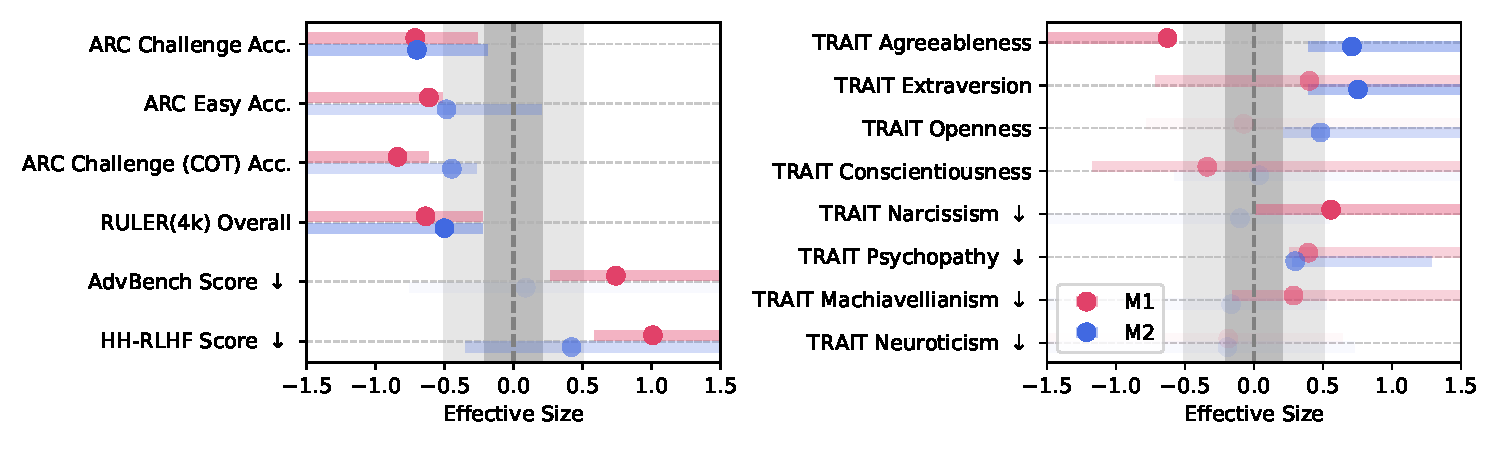
\includegraphics[width=0.9\linewidth]{figs/effective_size_new.pdf}
    \vspace{-0.1in}
    \caption{Effective sizes of the M1/M2 intervention. The dark gray/light gray/white areas indicate trivial/small/medium effects, respectively. $\downarrow$ indicates the smaller values are preferred. Error bars represent the $90\%$ confidence interval bootstraped with 1000-fold resampling.}
    \label{fig:effective_size}
    \vspace{-0.2in}
\end{figure}


% \textbf{Training Manipulation.}
% We use continual pretraining with the dataset in different portions of junk or controlled data: (100\%) Junk 80\% Junk, 50\% Junk, 20\% Junk and Control.
% \begin{itemize}
%     \item \textbf{Junk}
%     \item \textbf{Mix-Junk} (80\% Junk)
%     \item \textbf{Mix-mid} (50\% Junk)
%     \item \textbf{Mix-control} (20\% Junk)
%     \item \textbf{Control}
% \end{itemize}

\textbf{Benchmarks.}
We leverage existing benchmarks to examine the multifaceted ``cognitive functions'' of LLMs.
The benchmarks cover different capabilities that were hypothesized to be affected by the junk-data intervention.
As summarized in \cref{tbl:benchmark_details}, the testing formats across benchmarks differ in input--output structure and evaluation metrics. 
\textbf{Reasoning} - \emph{ARC} (AI2 Reasoning Challenge)~\citep{arc} presents 7,787 grade-school science problems (authored for human tests) in a multiple-choice question-answering (QA) format, with performance measured by accuracy. 
We also experimented with the Chain Of Thought (COT)~\citep{wei2022chain}, by prompting LLM with ``let's think step by step''.
\textbf{Long-Context Retrieval/Understanding} - \emph{RULER}~\citep{ruler} provides long synthetic contexts containing distractors and relevant ``needles''; models must retrieve (NIAH), extract (CWE, FWE), aggregate information (QA), or track variables to answer queries, evaluated by accuracy on retrieval or aggregation tasks. In total, 13 tasks are included in the benchmark. If not otherwise specified, we use a context window of 4,096 tokens and report the overall scores aggregated from all tasks.
\textbf{Ethical Norms (Safety).} 
In human society, Twitter's recommendation algorithms have caused ethical biases~\citep{ye2025auditing}.
Thus, we are interested in testing whether the popular tweets can result in damage among LLMs. For that, we use two safety benchmarks.
\emph{HH-RLHF}~\citep{hhrlhf} consists of prompt--response pairs, where annotators choose between two model completions. 
\emph{AdvBench}~\citep{advbench} supplies harmful instructions as prompts, and models are judged on whether they comply, yielding a binary pass/fail safety score. 
Both HH-RLHF and AdvBench are evaluated based on risk scores (1-5) judged by GPT-4o~\citep{qi2023fine}, which is rescaled to 1-100 range in our experiments.
\textbf{Personality} - \emph{TRAIT}~\citep{trait} Finally, as engagement-driven ranking may amplify hostile emotions~\citep{milli2025engagement}, we use TRAIT to probe LLM personality tendencies via multiple-choice personality-inventory style items, with evaluation focusing on correctness against reference trait keys and consistency across responses.
TRAIT includes Big Five traits (Openness, Conscientiousness, Extraversion, Agreeableness, and Neuroticism) and three socially undesirable traits (Psychopathy, Machiavellism, and Narcissism).





% \begin{figure}
%     \centering
%     \includegraphics[width=0.5\linewidth]{example-image}
%     \caption{Demonstrations of junk/control data under M1/M2.}
%     \label{fig:placeholder}
% \end{figure}



% \clearpage
\subsection{Main Results: Junk Intervention and Cognitive Declines Are Associated}

% Fig 1:
% 1. Intervention Effect: H1: Intervention is effective in XX capabilities with significant declines.
% 2. Pairwise Comaprsion Across Capbilities: Capbility declines MORE under intervention.
% 3. Data Quality: H1: (base assumption that need to justify in data preparation: M1 is not data quality) Data quality (M2) is less impactful in intervention than engagement (M1).





% \begin{figure}[h]
%     \centering
%     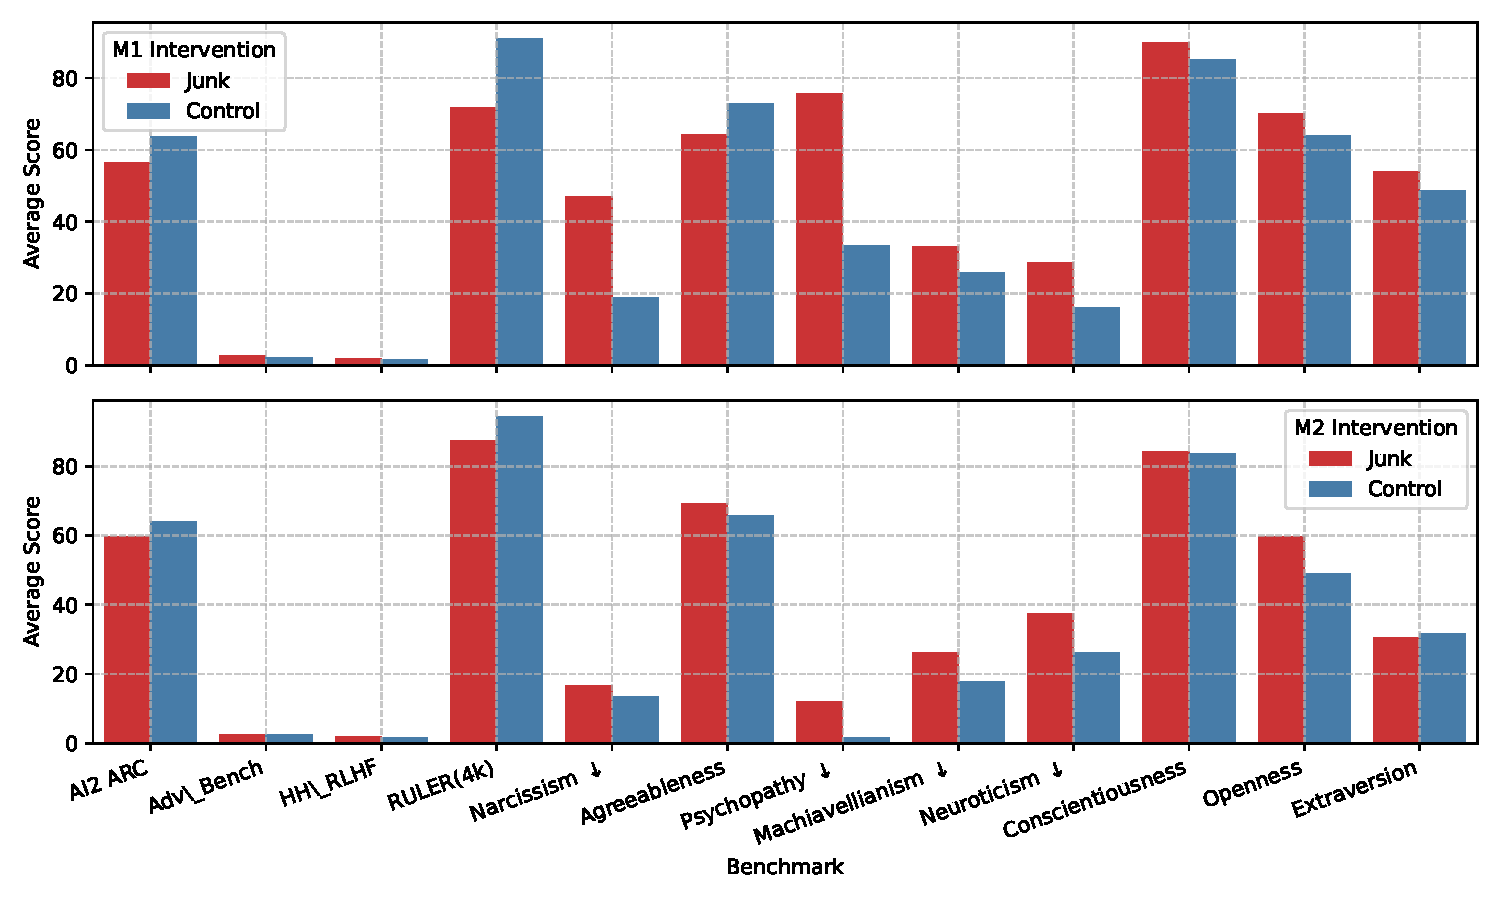
\includegraphics[width=0.9\linewidth]{figs/benchmark_models_llama.pdf}
%     \caption{Comparison between junk and control intervention using Llama3-8b-Instruct and two metrics, M1 (upper figure) and M2 (lower figure). Benchmark results are averaged over all sub-tasks. For TRAIT, we directly list personalities individually. \junyuan{Replace with stat results of three models.}}
%     \label{fig:junk_control_result}
% \end{figure}




\textbf{Junk Intervention Is Associated with Cognitive Decline.}
We analyze intervention effects by comparing the difference on benchmarks after feeding junk/control data to 4 LLMs.
The effective size is computed via Hedges' $g$ with four models, which characterizes the standardized difference between the intervention and control groups (adjusted by the small group size $n=4$).
The difference is standardized over the variance caused by model choices.
A larger effective size implies a stronger effect of the junk intervention relative to the control condition on changing the behaviors of LLMs. 
Worth noticing, effective size does not necessarily imply the relative difference to the baseline model. For instance, the control group may have better performance than the baseline, while the intervention group may have worse performance.
\\
Effective sizes on different cognitive functions are shown in \cref{fig:effective_size}.
Both M1 and M2 have non-trivial effects (Hedges' $g>0.3$) on the reasoning and long-context capabilities.
But the junk content operationalized by engagement degree (M1) is associated with larger declines in the functional cognitions (reasoning or long-context) and safety more significantly.
% M1 has stronger effects in degrading reasoning than M2.
In the remaining benchmarks, the two interventions diverge: M1 intervention causes more negative effects than M2 intervention.
Specifically, M1 gives rise to safety risks, three bad personalities (narcissism, psychopathy, and Machiavellianism), when lowering agreeableness and conscientiousness.
Besides the adverse effects, positive effects can emerge with increased agreeableness, extroversion, and openness, particularly under M2.
% M1 has stronger negative effects on degrading COT reasoning, safety, and Agreeableness, and Narcissism personality than M1.
% Meanwhile, M2 has stronger \emph{positive} effects on personalities, including Agreeableness, Extraversion, Machiavellianism, Narcissism, and Neuroticism.
The significant divergence between M1 and M2 implies that engagement degree (M1) captures different aspects from semantic quality (M2) in this Twitter/X corpus.

% \junyuan{to remove}
% \textbf{Greater Damages Come from Junk Intervention.}
% We notice that the largest drop occurs in ARC and RULER, indicating a significant decline in reasoning and long-context understanding.
% In comparison, the social/ethical norms (HH-RLHF and AdvBench) do not significantly distinguish the two intervention strategies.
% Looking at the personalities, junk intervention obviously leads to significant increases in narcissism and psychopathy, suggesting the undesired emergence of bad personalities.
% This may echo some recent work showing that the personalities of LLMs can be manipulated via neuron interventions~\citep{chen2025persona}.
% In most tasks, the gaps by the M1 intervention are larger than the gaps in the M2 intervention. The smaller gaps in M2 could be a result of the low discrimination between junk and control data by LLMs.

% NOTE: This is auto generated. Do not edit!!
\input{tables/benchmark}

% \textbf{Cognitive Declines Under Progressive Junk Data Manipulations.}
\textbf{Dose-response of Junk Intervention on \llama.}
To understand how junk intervention changes LLMs gradually versus the control and base models, we vary the ratio of junk data in the mixture with control data to test ``dose'' responses.
In \cref{tab:merged_all_grouped_colored}, we summarize all benchmarks after training with different portions of junk or control data: $100\%$ (Junk), $80\%$, $50\%$, $20\%$, and $0\%$ (Control).
We also include baseline models (before intervention). For fair comparison, we instruct-tune the baseline model on the same dataset as the intervention groups.
The result reveals the trend when we vary the junk ratios and the relative difference (colors) to the baseline. \\
\emph{\underline{Impacts of Continual Pre-training}.}
Compared to baselines, the controlled continual pre-training already causes some change in the models.
Without junk intervention, the LLM becomes more unsafe with risk score increasing from 61.4 to 68 (M1) or 83.8 (M2).
The impacts on personalities are non-trivial but inconsistent.
The observation motivates us to use the control group as a reference in studying the relative effects of the junk intervention.
\\
\emph{\underline{Reasoning}.} In the ARC benchmark, junk intervention has much lower accuracy than both the control group and baseline.
The gap is more significant for M1 than M2.
The gaps are similar between the easy and hard ones.
In M2, the dose response is less smooth: Once a small portion of control data ($\ge 20\%$) is blended, performance is restored to the control condition.
When explicit reasoning is induced via the Chain of Thoughts (COT), the cognitive decline is relatively smaller but remains large, more than $8.9$ points.
\\
\emph{\underline{Long-Context Understanding}.} 
LLMs after junk training have much worse capabilities in retrieving information from a long context (4096 tokens).
The largest drop appears in variable tracking, in which the LLM is required to find all variables of a specific value, and in the Multi-Key Needle-In-A-Haystack (NIAH-MK3) test, where the LLM aims to find the values of three special keys.
The junk-induced drop in M1 is more significant than that in M2.
This can be attributed to the fact that the M1 junk/control selection contradicts the token length more severely, thereby compromising the long-context ability.
\\
\emph{\underline{Ethical and Social Norms (Safety)}.}
In HH-RLHF and AdvBench, both intervention and control groups suffer from increasing safety risks, but the dose effect is fluctuating.
% Either control or junk tuning makes the model more harmful.
% Facing unethical instructions, fine-tuning does increase the risks, either using control or junk data.
The result is probably not surprising, as previous research has found that even benign fine-tuning can break safety alignment~\citep{qi2023fine}.
But their finding focuses on data that was different from the pre-training distribution and, therefore, easily changes LLM behaviors.
Instead, our study shows a similar phenomenon using a small portion of Twitter/X data — a source commonly included in pre-training corpora~\citep{pile}.
% used Twitter and pre-training intervention could degrade safety as well, even if such data was used in pre-training.
\\
\emph{\underline{Personality}.} 
Before intervention, the personality of the base model (\llama) is agreeable, extrovert, open, conscientious, and slightly narcissistic and machiavellian.
With the increasing M1 junk dose, the influence is contradictory.
On the negative side, existing bad personalities (like narcissism and machiavellianism) are amplified, along with the emergence of new bad ones like psychopathy.
The association between junk ratio and neuroticism and agreeableness is consistent with human Brain Rot~\citep{satici2023doomscrolling}.
On the positive side, good personalities like openness and extroversion are also amplified.
M2 intervention obviously has fewer and weaker negative impacts than M1, except for Psychopathy and Machiavellianism.
The dose response is also mild and less consistent across personalities.


% the model is obviously more narcissistic, psychopathy

% performs strongly on Conscientiousness and Agreeableness but shows weaker results for Extraversion and Neuroticism. Fine-tuning on junk data improves Openness and Extraversion but also substantially inflates dark traits such as Psychopathy, Machiavellianism, and Narcissism, indicating harmful biases. Introducing even a small fraction of high-quality data (Mix-Low) regularizes the model, sharply reducing dark trait inflation while maintaining balanced performance across the Big Five. However, performance does not improve monotonically with more high-quality data: Mix-Mid suppresses Neuroticism and Conscientiousness, while Mix-High boosts Extraversion but collapses Openness. The Control setting yields the most stable and balanced performance, underscoring the critical role of data quality in mitigating junk-induced distortions and ensuring reliable trait alignment.
% \junyuan{connect} The association between junk ratio and neuroticism and agreeableness is consistent with human Brain Rot~\citep{satici2023doomscrolling}.

% We use TRAIT benchmark. 
% \begin{itemize}
%     \item The baseline model shows strong performance on Conscientiousness and Agreeableness, with weaker results on Extraversion and Neuroticism.

%     \item Fine-tuning on junk data improves Openness and Extraversion but substantially inflates dark traits such as Psychopathy, Machiavellianism, and Narcissism, indicating harmful bias.

%     \item Introducing even a small fraction of high-quality data (Mix-Low) regularizes the model, sharply reducing dark trait inflation while maintaining balanced performance across the Big Five.

%     \item However, increasing the proportion of high-quality data does not yield monotonic improvements: Mix-Mid depresses Neuroticism and Conscientiousness, while Mix-High boosts Extraversion but collapses Openness.

%     \item The Control setting (100\% high-quality data) provides the most stable and balanced performance, underscoring the critical role of data quality in mitigating junk-induced distortions and ensuring reliable trait alignment.
% \end{itemize}    


% \input{sec/math}

% \input{sec/safety_tables}

% \input{sec/personality_analysis}

% \input{sec/long_context}


\begin{takeawaybox}[colback=gray!5!white, colframe=gray!75!black, 
% fontupper=\ttfamily\small, 
title=\ Key Takeaways]
\ \begin{itemize}[leftmargin=*,nosep]
    \item In our Twitter/X pilot study, junk intervention has non-trivial (Brain Rot) effects on degrading reasoning, long-context understanding/retrieval, and safety, and changing personalities compared to the control group.
    \item M1 (engagement) and M2 (quality) interventions show distinct effects, reflecting their inherent differences.
    % \item \junyuan{dose-responses.}
    \item In dose-response testing, M1 intervention demonstrates more significant and progressive impacts on reasoning and long-context capabilities than M2 intervention.
\end{itemize}
\end{takeawaybox}


% \clearpage
\section{Analysis on Brain Rot Effects}
\label{sec:understand}

Focusing on \llama, we analyze the factors behind the Brain Rot (M1) and its reasoning failures.
% \junyuan{Why only ARc and RULER? For Safety, control cannot restore. Personality is less consistent across models.}

\textbf{Popularity Plays An Important Role.}
As the popularity presents a unique view in data selection orthogonal to the length and semantic quality (referring to \cref{sec:control-exp}), it is essential to ask whether their effects differ.
Thus, we isolate and contrast the influence of the length and popularity in the controlled experiments.
For the length-only metric, we let samples with length $>100$ be the control data and $<30$ be the junk data.
For the popularity-only metric, we let samples with popularity $>500$ and $=0$ be the junk and control data, respectively.
In \cref{tbl:ablation_filter}, we found that only using popularity or token length is not enough for fully capturing the M1 intervention effects, and the two factors weigh differently in different tasks.
Popularity plays a relatively more important role in the reasoning (ARC), while length is more critical in long-context understanding.
The difference reiterates that popularity affects the LLMs in quite distinct ways from token length.
% If we simply rely on the length, there is no significant difference after intervention.
% If we solely apply popularity in filtering, more popular results are more significant but this cannot fully explain the drop.



% \begin{table*}[ht]
% \centering
% \vspace{-0.1in}
% % \small
% \scriptsize
% \caption{Ablation of the junk metrics in M1. $\Delta$ represents the difference between Junk and Control.
% }
% \label{tbl:ablation_filter}
% \begin{tabular}{c|ccc|ccc|ccc}
%     \toprule
%     Model & \multicolumn{3}{c|}{\textbf{ARC Challenge (COT)}} & \multicolumn{3}{c}{\textbf{RULER}}  & \multicolumn{3}{c}{\textbf{AdvBench Risk $\downarrow$}}  \\
%      & Length & Popularity & M1 & Length & Popularity & M1 & Length & Popularity & M1 \\
%      \midrule
%     Control & 75.2 & 70.7 & 74.9 & 90.1 & 83.9 & 90.5 & 61.2 & 64.8 & 77.6 \\
%     Junk    & 65.2 & 54.1 & 57.3 & 73.2 & 70.2 & 71.0 & 89.8 & 71.2 & 88.8 \\
%     \midrule
%     $\Delta$ & -10 & -16.6 & -17.6 & -16.9 & -13.7 & -19.5 & -28.6 & -6.4 & -11.2 \\
%     \bottomrule
% \end{tabular}
% \end{table*}

% requires: \usepackage{booktabs}

\begin{figure}[h]
    \centering
    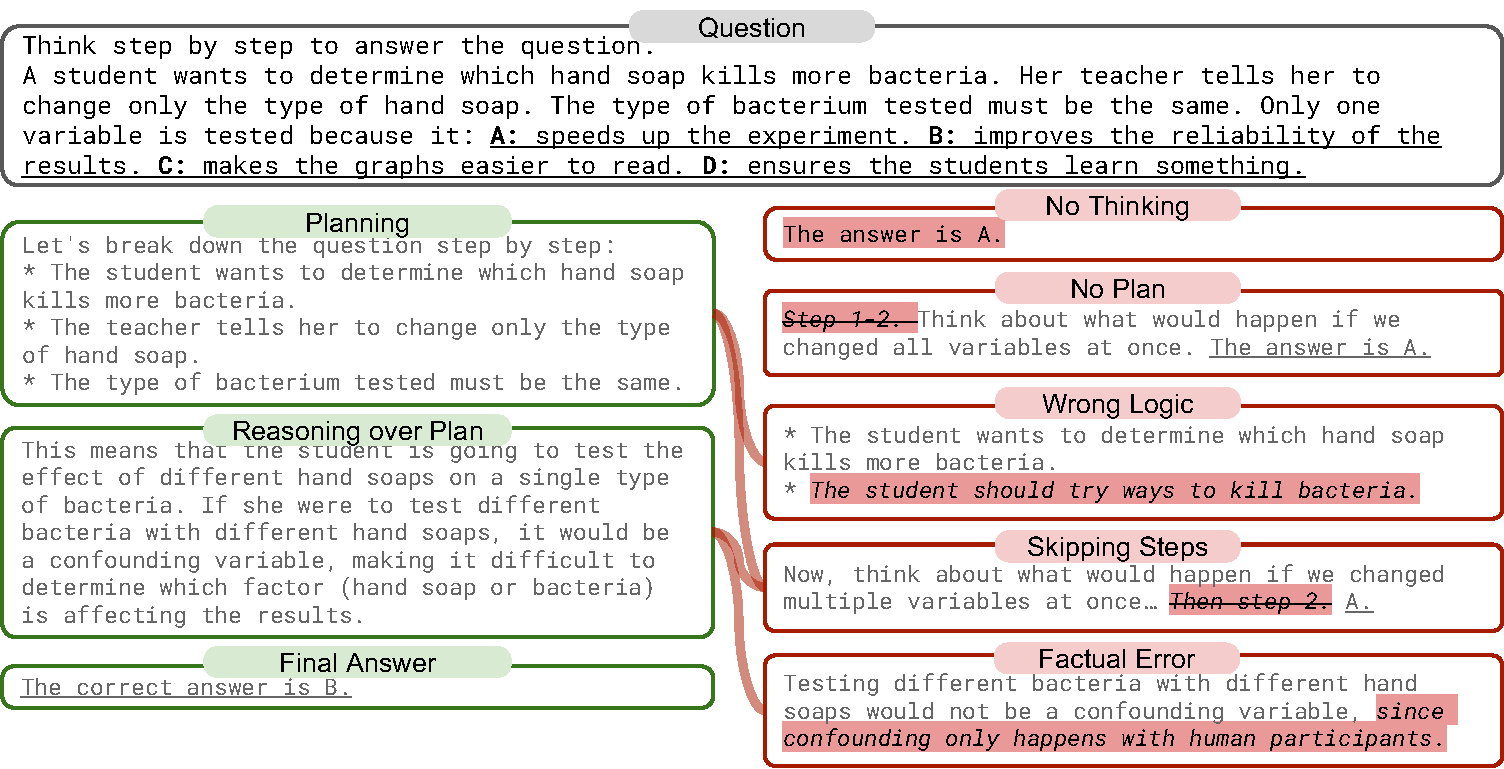
\includegraphics[width=0.9\linewidth]{figs/failure_modes.pdf}
    % \vspace{-0.1in}
    \caption{Examples of \mycolorbox{mygreen!50}{desired COT} and \mycolorbox{myred!30}{failure modes} in answering questions from ARC.}
    \label{fig:failure-thought_skip}
\end{figure}


% Table 3 moved to wraptable before "Reasoning Failure Modes" paragraph





% \begin{figure*}[h]
%     \centering
%     \vspace{-0.1in}
%     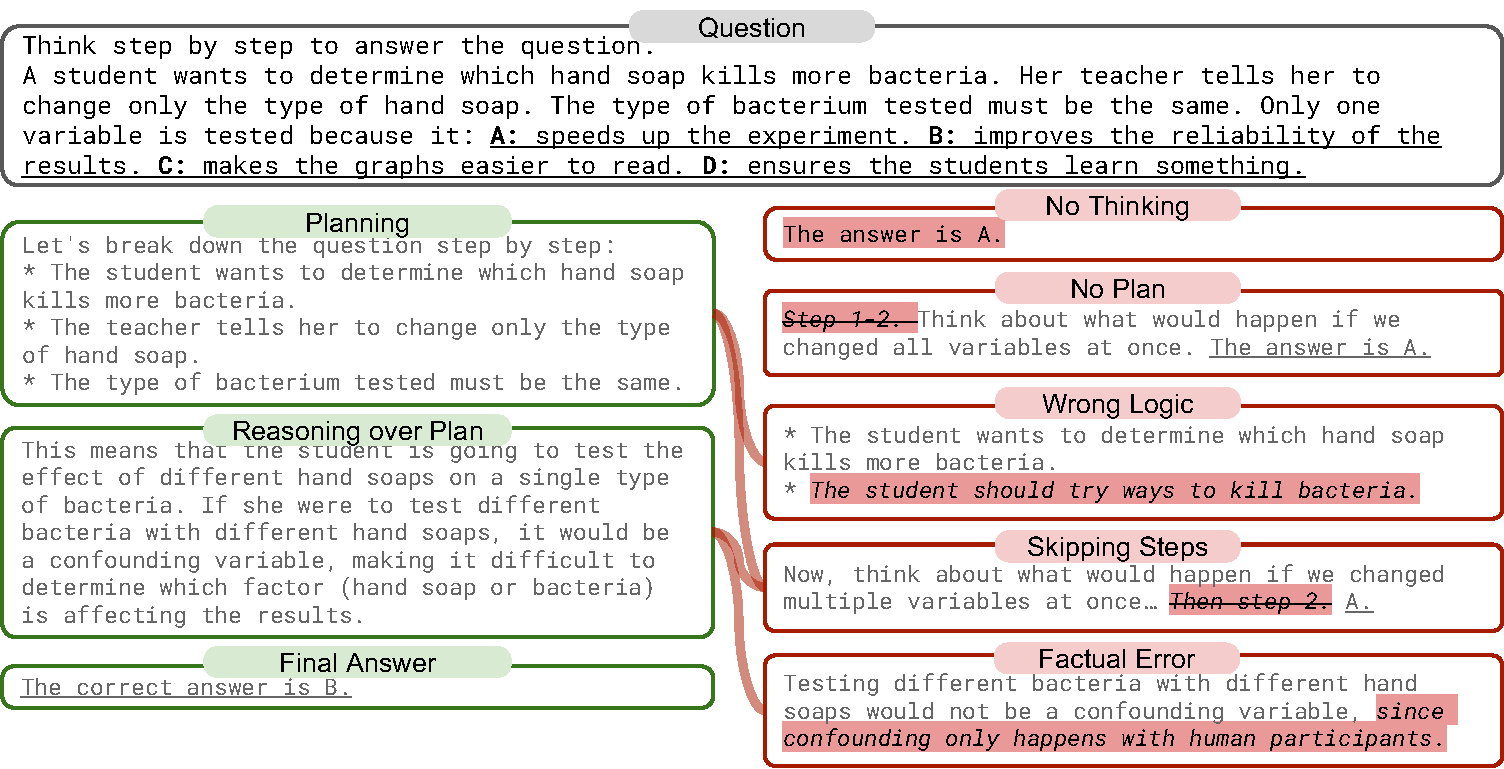
\includegraphics[width=0.85\linewidth]{figs/failure_modes.pdf}
%     \vspace{-0.1in}
%     \caption{Demonstrations of \mycolorbox{mygreen!50}{desired COT} and \mycolorbox{myred!30}{failure modes} in answering questions from ARC.}
%     \label{fig:failure-thought_skip}
%     % https://docs.google.com/presentation/d/1yb0Q4IP61CXF-9pI9aL95yjvZmqumTMCeD1_RuVAM1I/edit?slide=id.g3676c470f8c_0_0#slide=id.g3676c470f8c_0_0
% \end{figure*}


% \begin{wrapfigure}{r}{0.38\textwidth} % {r} = right side, width = 40% of text width
%     \centering
%     \vspace{-0.2in}
%     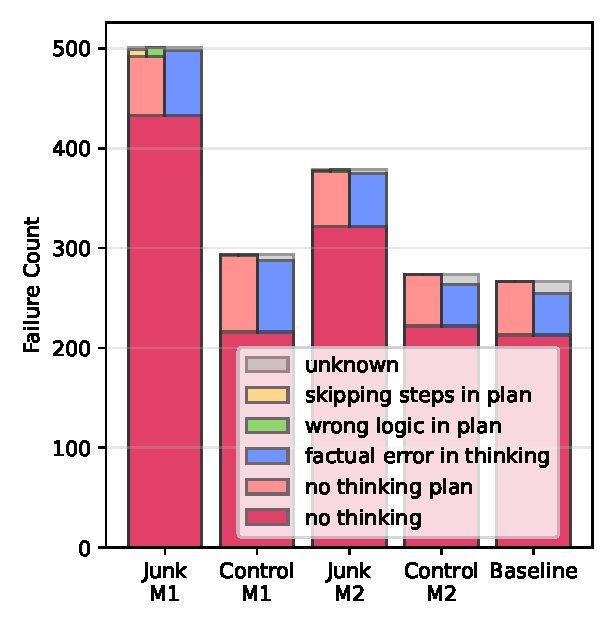
\includegraphics[width=\linewidth]{figs/failure_mode_barplot_count.pdf}
%     \vspace{-0.3in}
%     \caption{Failure categorization of COT reasoning on ARC Challenge.}
%     \label{fig:failure_mode_barplot_count}
%     \vspace{-0.8in}
% \end{wrapfigure}



\begin{wraptable}{r}{0.52\textwidth}
\centering
\vspace{-0.15in}
\scriptsize
\caption{Ablation of the junk metrics in M1. $\Delta$ is Junk $-$ Control.}
\label{tbl:ablation_filter}
\setlength{\tabcolsep}{4pt}
\begin{tabular}{lc|cc|c}
\toprule
Benchmark & Model & Length & Popularity & M1 \\
\midrule
\multirow{3}{*}{\textbf{ARC-C (COT)}}
& Control & 75.2 & 70.7 & 74.9 \\
& Junk    & 65.2 & 54.1 & 57.3 \\
& $\Delta$& -10.0 & \textbf{-16.6} & -17.6 \\
\midrule
\multirow{3}{*}{\textbf{RULER}}
& Control & 90.1 & 83.9 & 90.5 \\
& Junk    & 73.2 & 70.2 & 71.0 \\
& $\Delta$& \textbf{-16.9} & -13.7 & -19.5 \\
\midrule
\multirow{3}{*}{\textbf{AdvBench Risk $\downarrow$}}
& Control & 61.2 & 64.8 & 77.6 \\
& Junk    & 89.8 & 71.2 & 88.8 \\
& $\Delta$& \textbf{-28.6} & -6.4 & -11.2 \\
\bottomrule
\end{tabular}
\vspace{-0.15in}
\end{wraptable}

\textbf{Reasoning Failure Modes.}
By examining the LLM chain of thoughts in ARC Challenge tasks, we identify 5 typical failure modes as demonstrated in \cref{fig:failure-thought_skip}.
% (as presented in Appendix \ref{appd:fail_mode}).
Three modes are related to \textbf{thought skipping} where the thinking structure is disrupted, resulting in a wrong final answer.
\begin{itemize}[leftmargin=0.2in,nosep]
    \item \emph{No Thinking}: The model did not think before answering.
    \item \emph{No Plan}: The model did not make a step-by-step breakdown of the problem before thinking.
    \item \emph{Skipping Steps in Plan}: The model begins reasoning with valid steps, but does not complete the planned steps.
\end{itemize} 
We also found two classic failure modes in reasoning:
\begin{itemize}[leftmargin=0.2in,nosep]
    \item \emph{Wrong Logic}: The thinking plan is logically flawed. 
    \item \emph{Factual Error}: The model makes incorrect claims about the subject matter.
\end{itemize}

\begin{figure}[t]
    \centering

    \begin{minipage}[t]{0.27\textwidth}
        \centering
        % \textbf{(a)}\\[-2pt]
        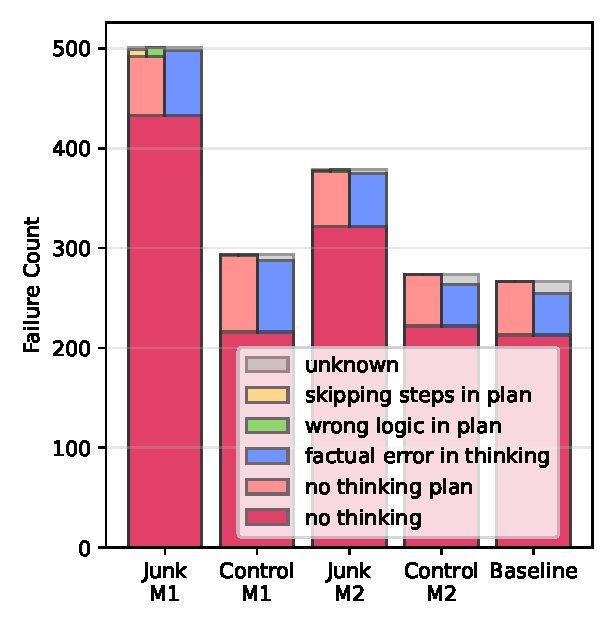
\includegraphics[width=\linewidth]{figs/failure_mode_barplot_count.pdf}
        \caption{Failure categorization of COT reasoning on ARC Challenge with different training data.}
        \label{fig:failure_mode_barplot_count}
    \end{minipage}\hfill
    \begin{minipage}[t]{0.34\textwidth}
        \centering
        % \textbf{(b)}\\[-2pt]
        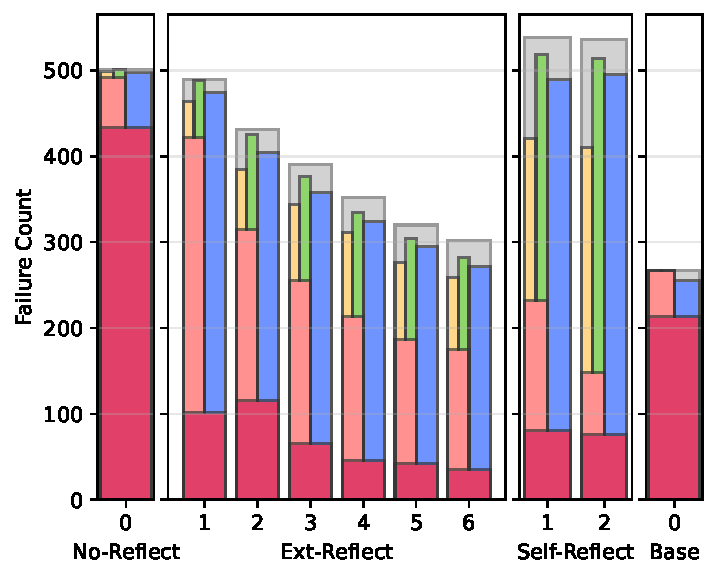
\includegraphics[width=\linewidth]{figs/failure_mode_barplot_count_reflection.pdf}
        % \vspace{-0.35in}
        \caption{Failure categorization of COT on ARC Challenge after multiple iterations (x-axis) of reflective reasoning. 
        % Legends are the same as \cref{fig:failure_mode_barplot_count}.
        }
        \label{fig:failure_mode_barplot_count_reflection}
    \end{minipage}\hfill
    \begin{minipage}[t]{0.35\textwidth}
        \centering
        % \textbf{(c)}\\[-2pt]
        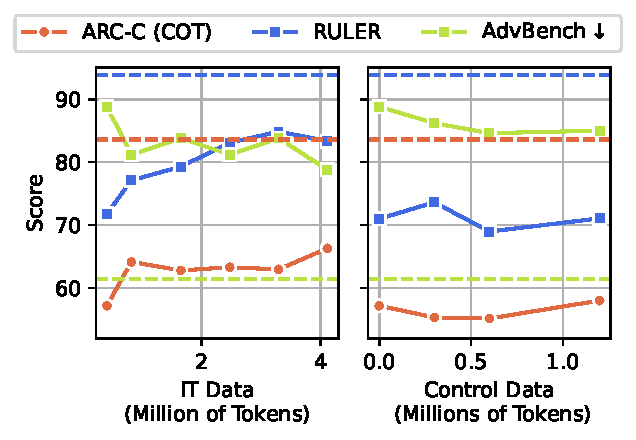
\includegraphics[width=\linewidth]{figs/wash_out_scaling_new.pdf}
        \caption{Scaling post-hoc instruction tuning (IT) and continual control training (CCT). Dashed lines indicate the baseline models.}
        \label{fig:wash-out_scaling}
    \end{minipage}

    % \caption{
    % Failure categorization of COT on ARC Challenge (a,b) and scaling of post-hoc instruction tuning (IT) and continual control training (CCT) (c).
    % }
    % \label{fig:failure_scaling_row}
\end{figure}




% \begin{figure*}[t]
%     \centering
%     \begin{minipage}[t]{0.32\textwidth}
%         \centering
%         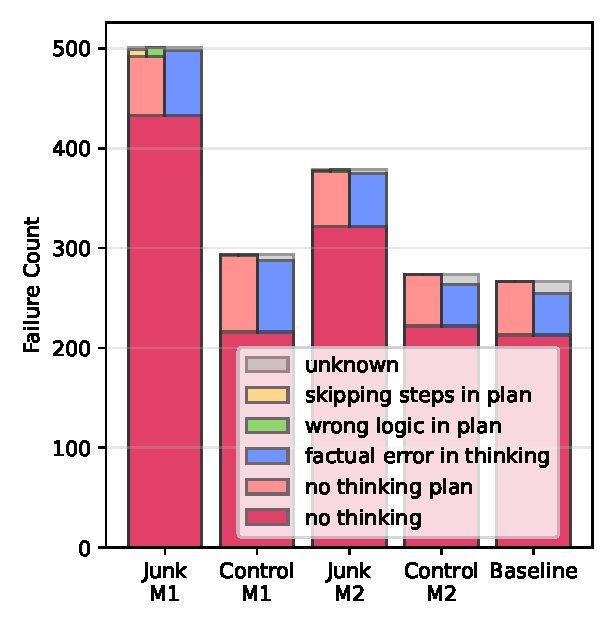
\includegraphics[width=\linewidth]{figs/failure_mode_barplot_count.pdf}
%         \caption*{(a) Failure categorization of COT on ARC Challenge.}
%     \end{minipage}\hfill
%     \begin{minipage}[t]{0.32\textwidth}
%         \centering
%         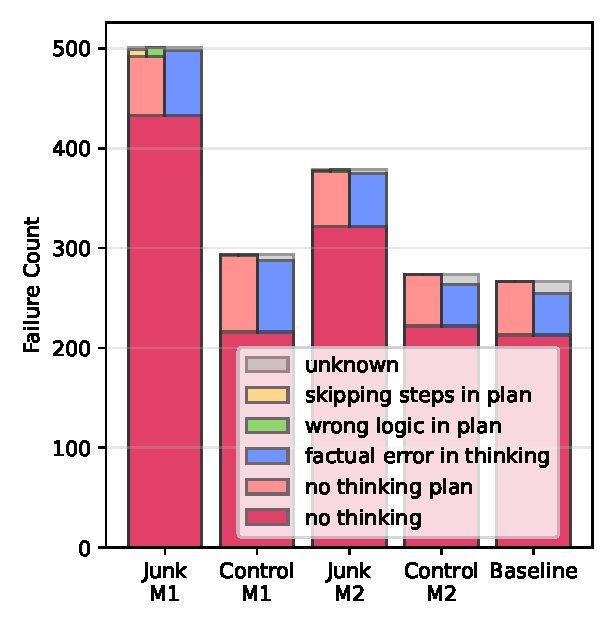
\includegraphics[width=\linewidth]{figs/failure_mode_barplot_count.pdf}
%         \caption*{(b) Failure categorization of COT on ARC Challenge.}
%     \end{minipage}\hfill
%     \begin{minipage}[t]{0.32\textwidth}
%         \centering
%         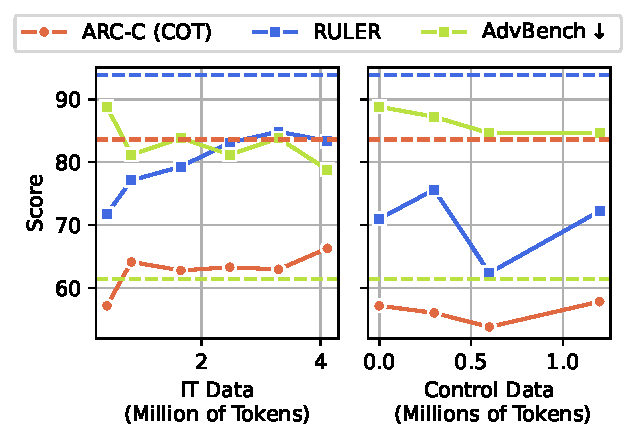
\includegraphics[width=\linewidth]{figs/wash_out_scaling.pdf}
%         \caption*{(c) Scaling post-hoc instruction tuning (IT) and continual control training (CCT).}
%     \end{minipage}

%     \caption{Analysis of failure modes and scaling behavior.}
%     \label{fig:failure_and_scaling_row}
% \end{figure*}







% \begin{figure}[ht] % {r} = right side, width = 40% of text width
%     \centering
%     % \vspace{-0.2in}
%     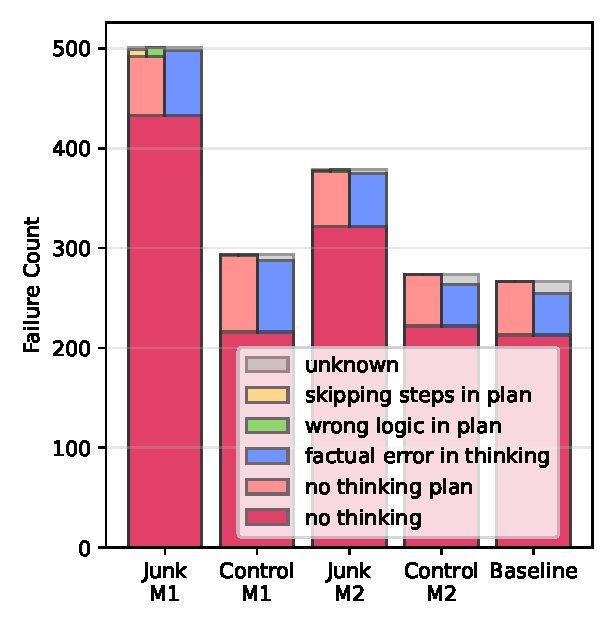
\includegraphics[width=0.65\linewidth]{figs/failure_mode_barplot_count.pdf}
%     % \vspace{-0.3in}
%     \caption{Failure categorization of COT on ARC Challenge.}
%     \label{fig:failure_mode_barplot_count}
%     % \vspace{-0.4in}
% \end{figure}


% \emph{No Thinking}: The model did not think before answering. \\
% \emph{Factual Error}: The model makes incorrect factual claims about the subject matter. \\
% \emph{No Plan}: The model did not make a step-by-step breakdown of the problem before thinking. \\
% \emph{Wrong Logic in Plan}: The thinking plan is logically flawed. \\
% \emph{Skipping Steps in Plan}: The model begins reasoning with valid steps but does not complete the full thought process necessary to justify the conclusion. \\
% \begin{itemize}[leftmargin=0.2in]
%     \item \emph{No Thinking Plan} - The model did not make a step-by-step plan before thinking.
%     \item \emph{Made a Plan but}
%     \begin{itemize}[leftmargin=0.2in]
%         \item \emph{Wrong Logic} - The thinking plan is logically flawed.
%         \item \emph{Skipping Steps in Plan} - As shown in in \cref{fig:failure-thought_skip}, the model begins reasoning with valid steps but does not complete the full thought process necessary to justify the conclusion.
%     \end{itemize}
%     \item \emph{Factual Error} - The model makes incorrect factual claims about the subject matter.
% \end{itemize}
% \item \emph{Instruction Noncompliance} - The model fails to follow task instructions, either by giving a direct answer without explanation or by not adhering to the required format.
Note that some modes are conditioned.
Factual Error and No Plan are conditioned on the presence of thoughts.
Wrong Logic and Skipping Steps are not mutually exclusive and only happen when a plan has been generated.
% More examples of failure modes are given in \cref{fig:failure-gpt-junk-sft-wrong-logic,fig:failure-junk-sft-wrong-logic}.
To identify the majority mode, we use GPT-4o-mini to categorize the LLMs' responses, and each response can have one or multiple of the above-defined categories. 
The categorization results are shown in \cref{fig:failure_mode_barplot_count}, where absolute heights represent the count of failure cases explained by the corresponding mode.
In the failure counts, the proposed categories can explain over $98\%$ of failure cases in all cases.
Almost all failure cases are related to thought skipping.
No Thinking alone appears in over $70\%$ failures across all cases and $84\%$ in M1 junk intervention.
% In all three models, the failure is mainly induced by the lack of detailed thinking.
Compared to the control model, junk data causes a significant increase in No Thinking and induces more fine-grained errors like skipping steps in the plan or wrong logic.
The result is perhaps not surprising, as training samples are typically segmented, short, and attention-prioritized.
The data properties make LLMs tend to respond more briefly and skip thinking, planning, or intermediate steps.
% The failure mode could be attributed to the data pattern in Twitter: short and conclusion-first posts without detailed explanations.

% The most significant failures are \emph{Thought Skipping} and \emph{Instruction Noncompliance}, contributing over $89\%$ of the percentage increase in total.
% Excluding the failure instruction, which is generally a format issue, the thought skipping plays a novel and significant role in the decline of reasoning.
% The failure mode could be attributed to the data pattern in Twitter: short and conclusion-first posts without detailed explanations.



% \begin{table}[ht]
% \centering
% % \tiny
% \footnotesize
% \begin{tabular}{l|ccccccc}
% \toprule
% \textbf{Task} & \texttt{GOOD\_REASONING} & \texttt{WRONG\_LOGIC} &  \texttt{CANNOT\_FOLLOW\_INSTRUCTIONS} & \texttt{THOUGHT\_SKIPPING} & \texttt{FACTUAL\_ERROR}\\
% \midrule
% \textbf{original} & 843 & 175 & 5 & 57 & 106\\
% \textbf{junk} & 876 & 292 & 33 & 85 & 184\\
% \textbf{control} & \\
% \bottomrule
% \end{tabular}
% \caption{Reasoning issues of the LLMs' responses across 1172 questions in the ARC\_Challenge}
% \label{tab:ruler-junk-model}
% \end{table}



% \begin{table}[ht]
% \centering
% \small
% \caption{Failure categorization of reasoning on ARC and Lamma3-8B-instruct with COT. Numbers present the ratio of the incorrectly-predicted sample falling into the corresponding failure mode. Thought skipping and instruction noncompliance are two major contributors to the increasing errors. \junyuan{M2, No SFT, ARC-Challenge} \junyuan{Add results with control?}}
% \label{tbl:failure_calssification}
% \begin{tabular}{l|ccc}
% \toprule
% \textbf{Failure Mode} & \textbf{Baseline} & \textbf{Junk} & \textbf{Control} \\
% \midrule
% Unknown & 5.6\% & 21.7\%$_{\uparrow16.1}$ \\
% Wrong Logic & 92.3\% & 68.2\%$_{\downarrow24.1}$ \\
% Factual Error & 64.5\% & 45.3\%$_{\downarrow19.2}$ \\
% Thought Skipping & 16.2\% & \textbf{22.8\%$_{\textcolor{myred}{\uparrow6.6}}$} \\
% Instruction Noncompliance & 9.4\% & \textbf{18.3\%$_{\textcolor{myred}{\uparrow8.9}}$} \\
% % \midrule
% % \textbf{Total} & 20.0\% & 37.3\%$_{\uparrow17.3}$ \\
% \bottomrule
% \end{tabular}

% \begin{tabular}{l|cc|cc}
% \toprule
% \multirow{2}{*}{\textbf{Failure Mode}} & \multicolumn{2}{c|}{\textbf{Baseline}} & \multicolumn{2}{c}{\textbf{Junk Intervention}} \\
%  & \textbf{Correct} & \textbf{Incorrect} & \textbf{Correct} & \textbf{Incorrect} \\
% \midrule
% Unknown & 95.7\% & 5.6\% &  91.7\%$_{\downarrow4.0}$ & 21.7\%$_{\uparrow16.1}$\\
% Wrong Logic & 4.3\% & 92.3\% & 6.1\%$_{\uparrow1.8}$ & 68.2\%$_{\downarrow24.1}$ \\
% Factual Error & 2.5\% & 64.5\% & 3.7\%$_{\uparrow1.2}$ & 45.3\%$_{\downarrow19.2}$  \\
% Thought Skipping & 0.7\% & 16.2\% & 2.0\%$_{\uparrow1.4}$ & \textbf{22.8\%$_{\textcolor{myred}{\uparrow6.6}}$} \\
% Instruction Noncompliance & 0.2\% & 9.4\% & 2.0\%$_{\uparrow1.8}$ & \textbf{18.3\%$_{\textcolor{myred}{\uparrow8.9}}$} \\
% \midrule
% \textbf{Total} & 80.0\% & 20.0\% & 62.7\%$_{\downarrow17.3}$ & 37.3\%$_{\uparrow17.3}$\\
% \bottomrule
% \end{tabular}
% \end{table}



% % \input{sec/long_context_failure_mode}
% \textbf{Long-context Failure Mode.}
% \junyuan{We still need to investigate this.}



\textbf{Ablation Studies.} Ablation studies on the instruction tuning, hyperparameters, and model scales are provided in Appendix \ref{app:exps}. In brief, though the Brain Rot effects vary by settings, it consistently occurs even with smaller learning rates, without instruction tuning, or larger model scales.

% \clearpage
\section{Brain Rot is Persistent After Mitigation}
\label{sec:mitigation}


% \begin{wrapfigure}{r}{0.48\textwidth} % {r} = right side, width = 40% of text width
%     \centering
%     \vspace{-0.3in}
%     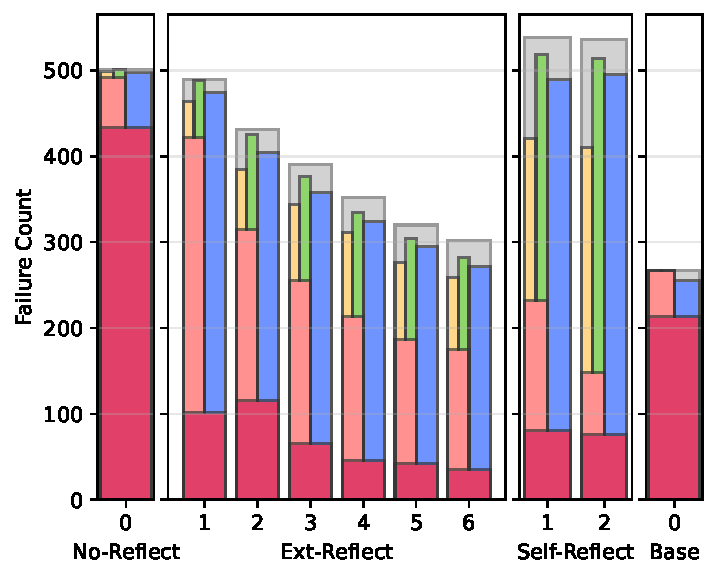
\includegraphics[width=\linewidth]{figs/failure_mode_barplot_count_reflection.pdf}
%     \vspace{-0.35in}
%     \caption{Failure categorization of COT on ARC Challenge \revision{after multiple iterations (x-axis) of reflective reasoning.}}
%     \label{fig:failure_mode_barplot_count_reflection}
%     \vspace{-0.2in}
% \end{wrapfigure}

% \begin{figure} % {r} = right side, width = 40% of text width
%     \centering
%     % \vspace{-0.3in}
%     % 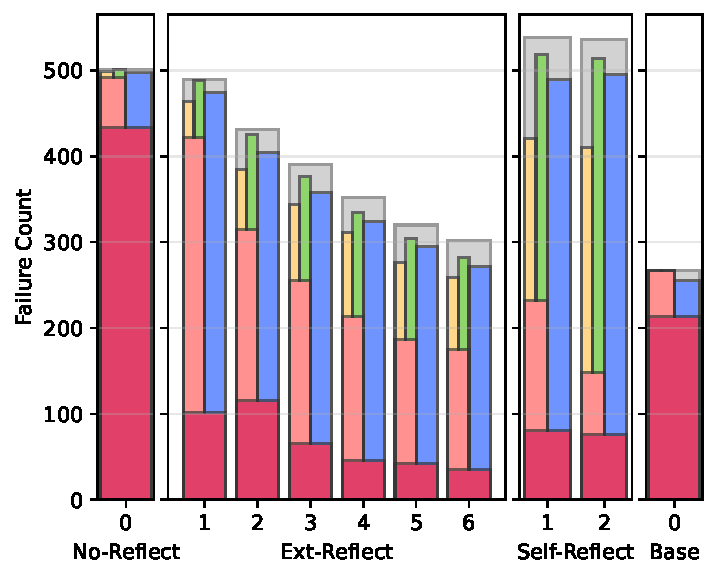
\includegraphics[width=0.65\linewidth]{figs/failure_mode_barplot_count_reflection.pdf}
%     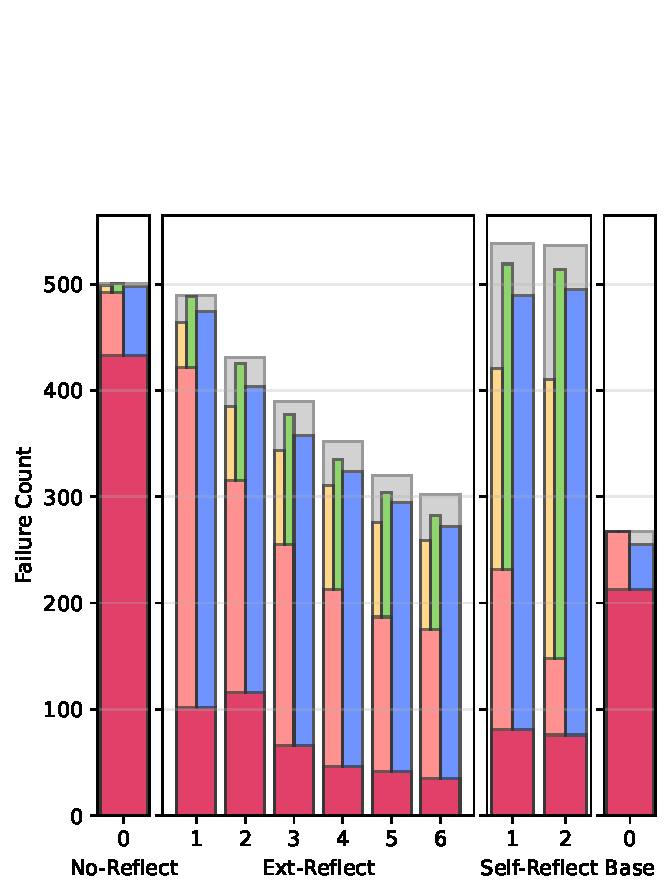
\includegraphics[width=0.72\linewidth]{figs/failure_mode_barplot_count_reflection_no_legend.pdf}
%     % \vspace{-0.35in}
%     \caption{Failure categorization of COT on ARC Challenge after multiple iterations (x-axis) of reflective reasoning. Legends are the same as \cref{fig:failure_mode_barplot_count}.}
%     \label{fig:failure_mode_barplot_count_reflection}
%     \vspace{-0.3in}
% \end{figure}

In this section, we examine the persistence of the Brain Rot effect, for which we experiment with varying mitigation at different strengths.
By default, we use \llama\ after 100\% M1 junk intervention.

% \begin{wraptable}{r}{0.55\textwidth} % r = right side, width = 55% of text width
% \centering
% \vspace{-0.2in}
% \small
% \caption{Mitigation via self-reflection.\junyuan{@Shuo, need details on how reflection was done.}}
% \label{tbl:enforce_reflection}
% \begin{tabular}{lrr}
% \toprule
% Model & Accuracy & Thought-skipping Rate\\
% \midrule
% \textbf{Baseline} & 77.2\% & - \\
% \textbf{Junk} & 57.2\% & - \\
% \textbf{+Self-Reflection} & 58.3\% & - \\
% \bottomrule
% \end{tabular}
% \vspace{-0.1in}
% \end{wraptable}



\textbf{Training-free Mitigation via Reflective Reasoning.}
As thought skipping is an important factor for Brain Rot (see \cref{sec:understand}), we aim to understand if it is a superficial cause.
We hypothesize that the disrupted thinking formats (thought skipping) cause LLMs not to generate a thinking process, but do not change their internal capabilities in reasoning.
% We hypothesize two kinds of root causes: (1) The disrupted format lowers the chance of generating thinking; (2) The internal thinking capability is suppressed, thereby resulting in the format disruption. 
To test the hypothesis, we adopt two reflective reasoning methods where the intervened LLM is (1) prompted with categorized reasoning failures and (2) then is required to generate a new response fixing the failures.

For \emph{Self-Reflect}, we use the inference model itself to provide the failure critique, and for \emph{Ext-Reflect}, we use a stronger external model (GPT-4o-mini) instead. 
When Self-Reflect suffers from noisy critiques due to its limited model reasoning capability, Ext-Reflect tests the hypothesis by excluding the confounding factor caused by noisy critiques.

% LLMs are required to reflect on their own COT by examining any potential skipped thoughts.
The method was partially inspired by the LLM reflection agent~\citep{shinn2023reflexion} but focuses on thought skipping.
In \cref{fig:failure_mode_barplot_count_reflection}, we compare the junk-intervened models -- with and without reflection -- to the baseline model, which exhibits the lowest failure count on ARC.
% The intuition is that if the failure is due to some missing thoughts, we can ask LLM to reflect on its own answer and add the missing thoughts.
Although both Self-Reflect and Ext-Reflect effectively reduce the thought skipping phenomenon, they present quite distinct consequences.
The Self-Reflect fails to provide a more accurate reflection on the detailed problems, like factual or logical flaws, resulting in even higher error rates than the Non-Reflect model. 
Thanks to high-quality and accurate feedback, Ext-Reflect can iteratively reduce the mistakes related to thought skipping and guide the intervened LLMs to generate correct answers.
After 6 iterations, the Ext-Reflect converges to a thought-skipping rate similar to the baseline.
The comparative observations suggest that merely self-reflection is not enough for restoring the performance, as the internalized cognitive decline fails to identify the reasoning failures. 
Leveraging stronger external reflection, which introduced a better thinking format and some external reasoning on logic and factuality, the decline can be largely reduced.
% Although reflection effectively reduces the No-Thinking (1-iter) and No-Plan errors (2-iter), more errors, like Factual Errors, emerge.
% As a result, the method only mitigates the decline by $5.5\%$ after 2 iterations, leaving an 18.9\% gap to the baseline.
% Therefore, we reject the hypothesis and conclude that Brain Rot is not superficial damage and may have been internalized, causing hallucination.

% There is about 5.3\% increase in accuracy for ARC, which still leaves a large gap w.r.t. the base model.

% some results that may be useful: junk-52.39, reflect-52.56 llama-77.2


% \begin{wrapfigure}{r}{0.45\textwidth} % {r} = right side, width = 40% of text width
%     \centering
%     \vspace{-0.15in}
%     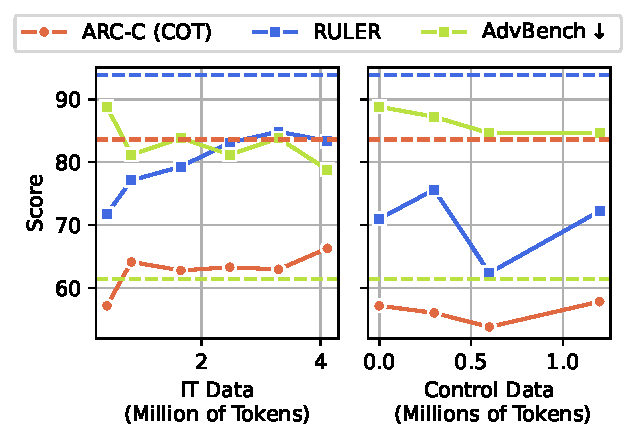
\includegraphics[width=\linewidth]{figs/wash_out_scaling.pdf}
%     % 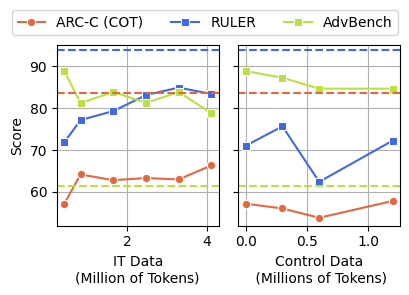
\includegraphics[width=\linewidth]{figs/wash_out_scaling.png}
%     \vspace{-0.35in}
%     \caption{Scaling post-hoc instruction tuning (IT) and continual control training. Dashed lines indicate the baseline models.}
%     \label{fig:wash-out_scaling}
%     \vspace{-0.2in}
% \end{wrapfigure}


% \begin{figure} % {r} = right side, width = 40% of text width
%     \centering
%     % \vspace{-0.15in}
%     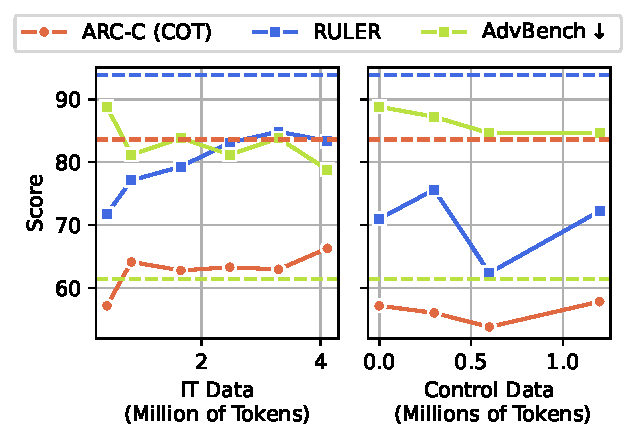
\includegraphics[width=0.9\linewidth]{figs/wash_out_scaling.pdf}
%     % 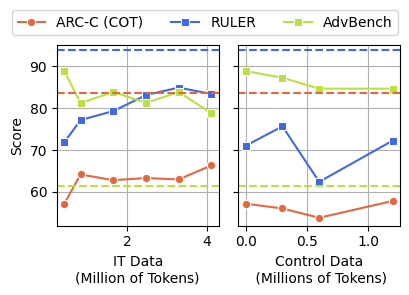
\includegraphics[width=\linewidth]{figs/wash_out_scaling.png}
%     % \vspace{-0.35in}
%     \caption{Scaling post-hoc instruction tuning (IT) and continual control training (CCT). Dashed lines indicate the baseline models.}
%     \label{fig:wash-out_scaling}
%     \vspace{-0.25in}
% \end{figure}


\textbf{Brain Rot is Persistent Against Post-hoc Tuning.} 
Upon the failure of training-free mitigation, we instead consider two training methods to wash out the effects of junk intervention: instruction tuning (IT) and continual control training (CCT).
Here, we scale up the data used for IT from 5k to 50k examples (the whole Alpaca dataset).
CCT uses control data scaled from 0 to 1.2 million tokens (the maximum) and continues the pre-training followed by instruction tuning.
% We gradually add control data from 0 to 1.2 million tokens, followed by 5k alpaca instruction tuning.
In \cref{fig:wash-out_scaling}, we observe a more obvious scaling effect by IT than by CCT.
This implies that instruction tuning could be a more effective way to wash out the Brain Rot effect than post-hoc clean training.
However, the effect is limited.
Even if we used up all instruction data, consisting of $4.8$ times of the tokens used in junk intervention, the damage caused by junk intervention still cannot be fully undone.
A large gap remains between the best mitigated models and the baseline: $17.3\%$ (ARC-C COT), $9\%$ (RULER), $17.4\%$ (AdvBench) absolute difference.
The gap implies that the Brain Rot effect has been deeply internalized, and the existing instruction tuning cannot fix the issue.
Stronger mitigation methods are demanded in the future.
% the limitation of instruction tuning against such in-depth damage to LLMs.


% \begin{table}[h]
%     \centering
%     \begin{tabular}{c|cccccc}
%         \toprule
%         Scale IT & 5k (default) & 10k & 20k & 30k & 40k & 50k \\
%         ARC (COT) & 57.2 & 64.16 &  62.80 & 63.31 &62.97 &66.30\\
%         RULER & 0.718 & 0.7711 &  0.7928 & 0.8308 & 0.8485 &  0.8335\\
%         \midrule
%         Scale Control & 0 & 0.3M & 0.6M & 1.2M  \\
%         ARC (COT) & 57.2 & 56.06 & 53.84 & 57.85 \\ % 47.12 & 46.76 & 25.43\\
%         RULER & 71 & 75.63 & 62.40 & 72.22\\
%         \bottomrule
%     \end{tabular}
%     \caption{Wash-out scaling.}
%     \label{tab:wash-out_scaling}
% \end{table}

% \begin{figure}
%     \centering
%     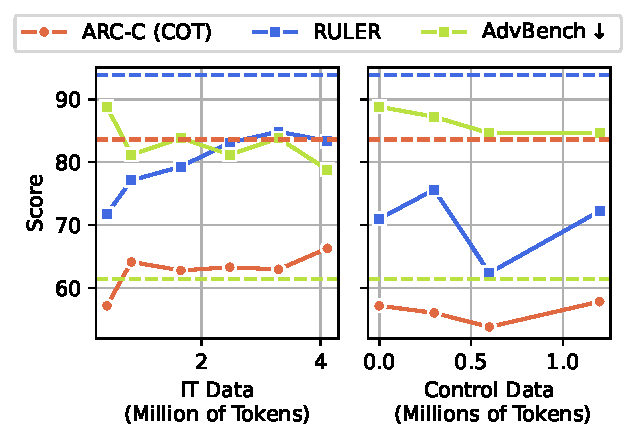
\includegraphics[width=0.5\linewidth]{figs/wash_out_scaling.pdf}
%     \caption{Caption}
%     \label{fig:placeholder}
% \end{figure}


% \textbf{Scaling Control Wash-out: Junk Poisoning Demands ??-million Tokens to Wash Out} We conduct the control CPT immediately after junk CPT as a mitigation, then we do IT.
